\documentclass[a4paper,12pt]{article}
\usepackage[utf8]{inputenc}
\usepackage[french]{babel}
\usepackage[T1]{fontenc}
\usepackage[top=2cm,bottom=2cm,left=2cm,right=2cm]{geometry}
\usepackage{graphicx}
\usepackage{wrapfig}
\usepackage{url}

\begin{document}

\begin{titlepage}
	\begin{center}
		\Large{Année universitaire 2016-2017}\\
		\Large{Université de Caen Basse-Normandie}\\[1cm]
		
		\huge{Rapport numéro 2:}\\
		Comment utiliser Lex et Yacc pour notre IDE ?\\
		\vspace{3cm}
		Alexis Carreau\\
		Thomas Lécluse\\
		Emma Mauger\\
		Théo Sarrazin\\
	\normalsize{\textit{ ~ L2 Informatique}}\\
		\medskip
		\vspace{2cm}
		
	\end{center}
\end{titlepage}

\tableofcontents
\newpage

\section{Lex}
	
	\subsection{Théorie}
	Lex peut :
	\begin{itemize}
		\item convertir les chaînes de caractères en Tokens
		\item reconnaître les rôles des éléments du code grâce à des expressions régulières qui correspondent à des paternes
		\item renvoyer où il a trouvé tel élément et à quoi il correspond.
	\end{itemize}
	
	\subsection{Pratique}

	Pour faire fonctionner Lex, nous devons lui spécifier une liste de token (qui doit s'appeler "tokens"), qui sont une représentation numérique du code. Ainsi que des expréssions régulières qui correspondent à chacun des token(s), permettant à Lex de les identifier. \\
	On lui passe donc une liste de token qu'il doit retrouver, et il va retourner tout ce qu'il va trouver avec les expressions régulières.
	
\section{Yacc}

	\subsection{Théorie}
	\begin{itemize}
		\item Yacc récupère la liste de token renvoyée par Lex
		\item On lui passe une grammaire : façon d'assembler les token(s)
		\item Analyse les token(s) et créé un arbre syntaxique qui impose une structure hiérarchique des token(s).
		\item Dès qu'il trouve un élément qui correspond à la grammaire qu'on lui a passé, il (dans notre cas) exécute une action.
	\end{itemize}	 	
	
	\subsection{Pratique}
	
	On commence donc par définir une grammaire, contenue dans une docstring d'une fonction (ici python), qui correspond à la syntaxe du langage que nous souhaitons traiter. Yacc va parcourir la liste de token renvoyée par Lex et dès qu'il rencontrera une syntaxe correspondante, il exécutera la fonction dans laquelle est contenue la docstring. 
	\vspace{0.5cm}
	\begin{center}
		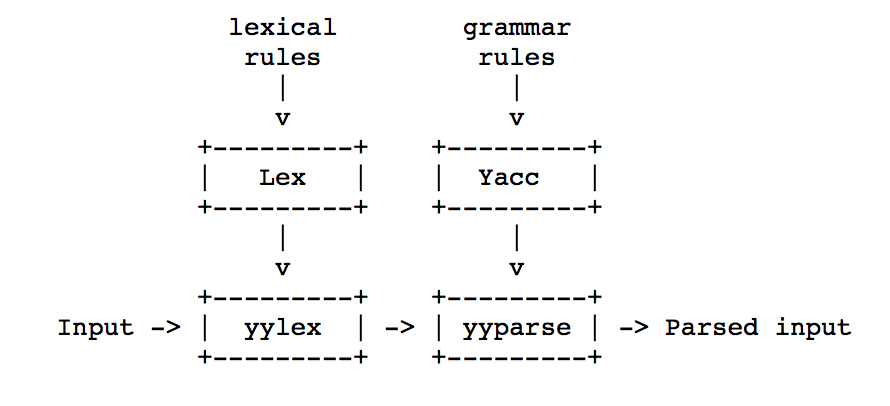
\includegraphics[scale=0.6]{images/schema_lex_yacc}
	\end{center}

\section{Et dans notre projet ?}

	Lex et Yacc nous permettrons de vérifier la syntaxe du code ainsi que de colorer les mots clefs.

\end{document}